\section{界面}

界面是一整块，从上到下五条带，从左到右三列。

\begin{enumerate}
\item 菜单条。文件、编辑、视图、样式、运行、数据、语言都在这一行，平铺不藏二级菜单。
\item 节点库。按工作流、数据输入、数据处理、结果输出四组排列，点一下把节点放到画布中央，也可以按住拖到指定位置。
\item 画布。网格底，节点在这里摆放与连线，滚轮缩放，空白处拖动平移，左下角有缩略图。
\item 大纲。当前画布的节点清单，点一条就把镜头移过去，节点多的时候靠它找路。
\item 停靠面板。控制台、进程监控、运行记录、定时任务、文献计量、导出产物、已保存的登录、数据集、词库、工作流文件都在这里，点底部的按钮打开，一次只开一个，再点一次收起。
\item 状态栏。节点数、预计行数、预计调用模型次数、缩放比例，运行前扫一眼能省不少等待。
\end{enumerate}

\begin{figure}[H]\centering
\begin{tikzpicture}
\node[anchor=south west,inner sep=0] (shot) at (0,0) {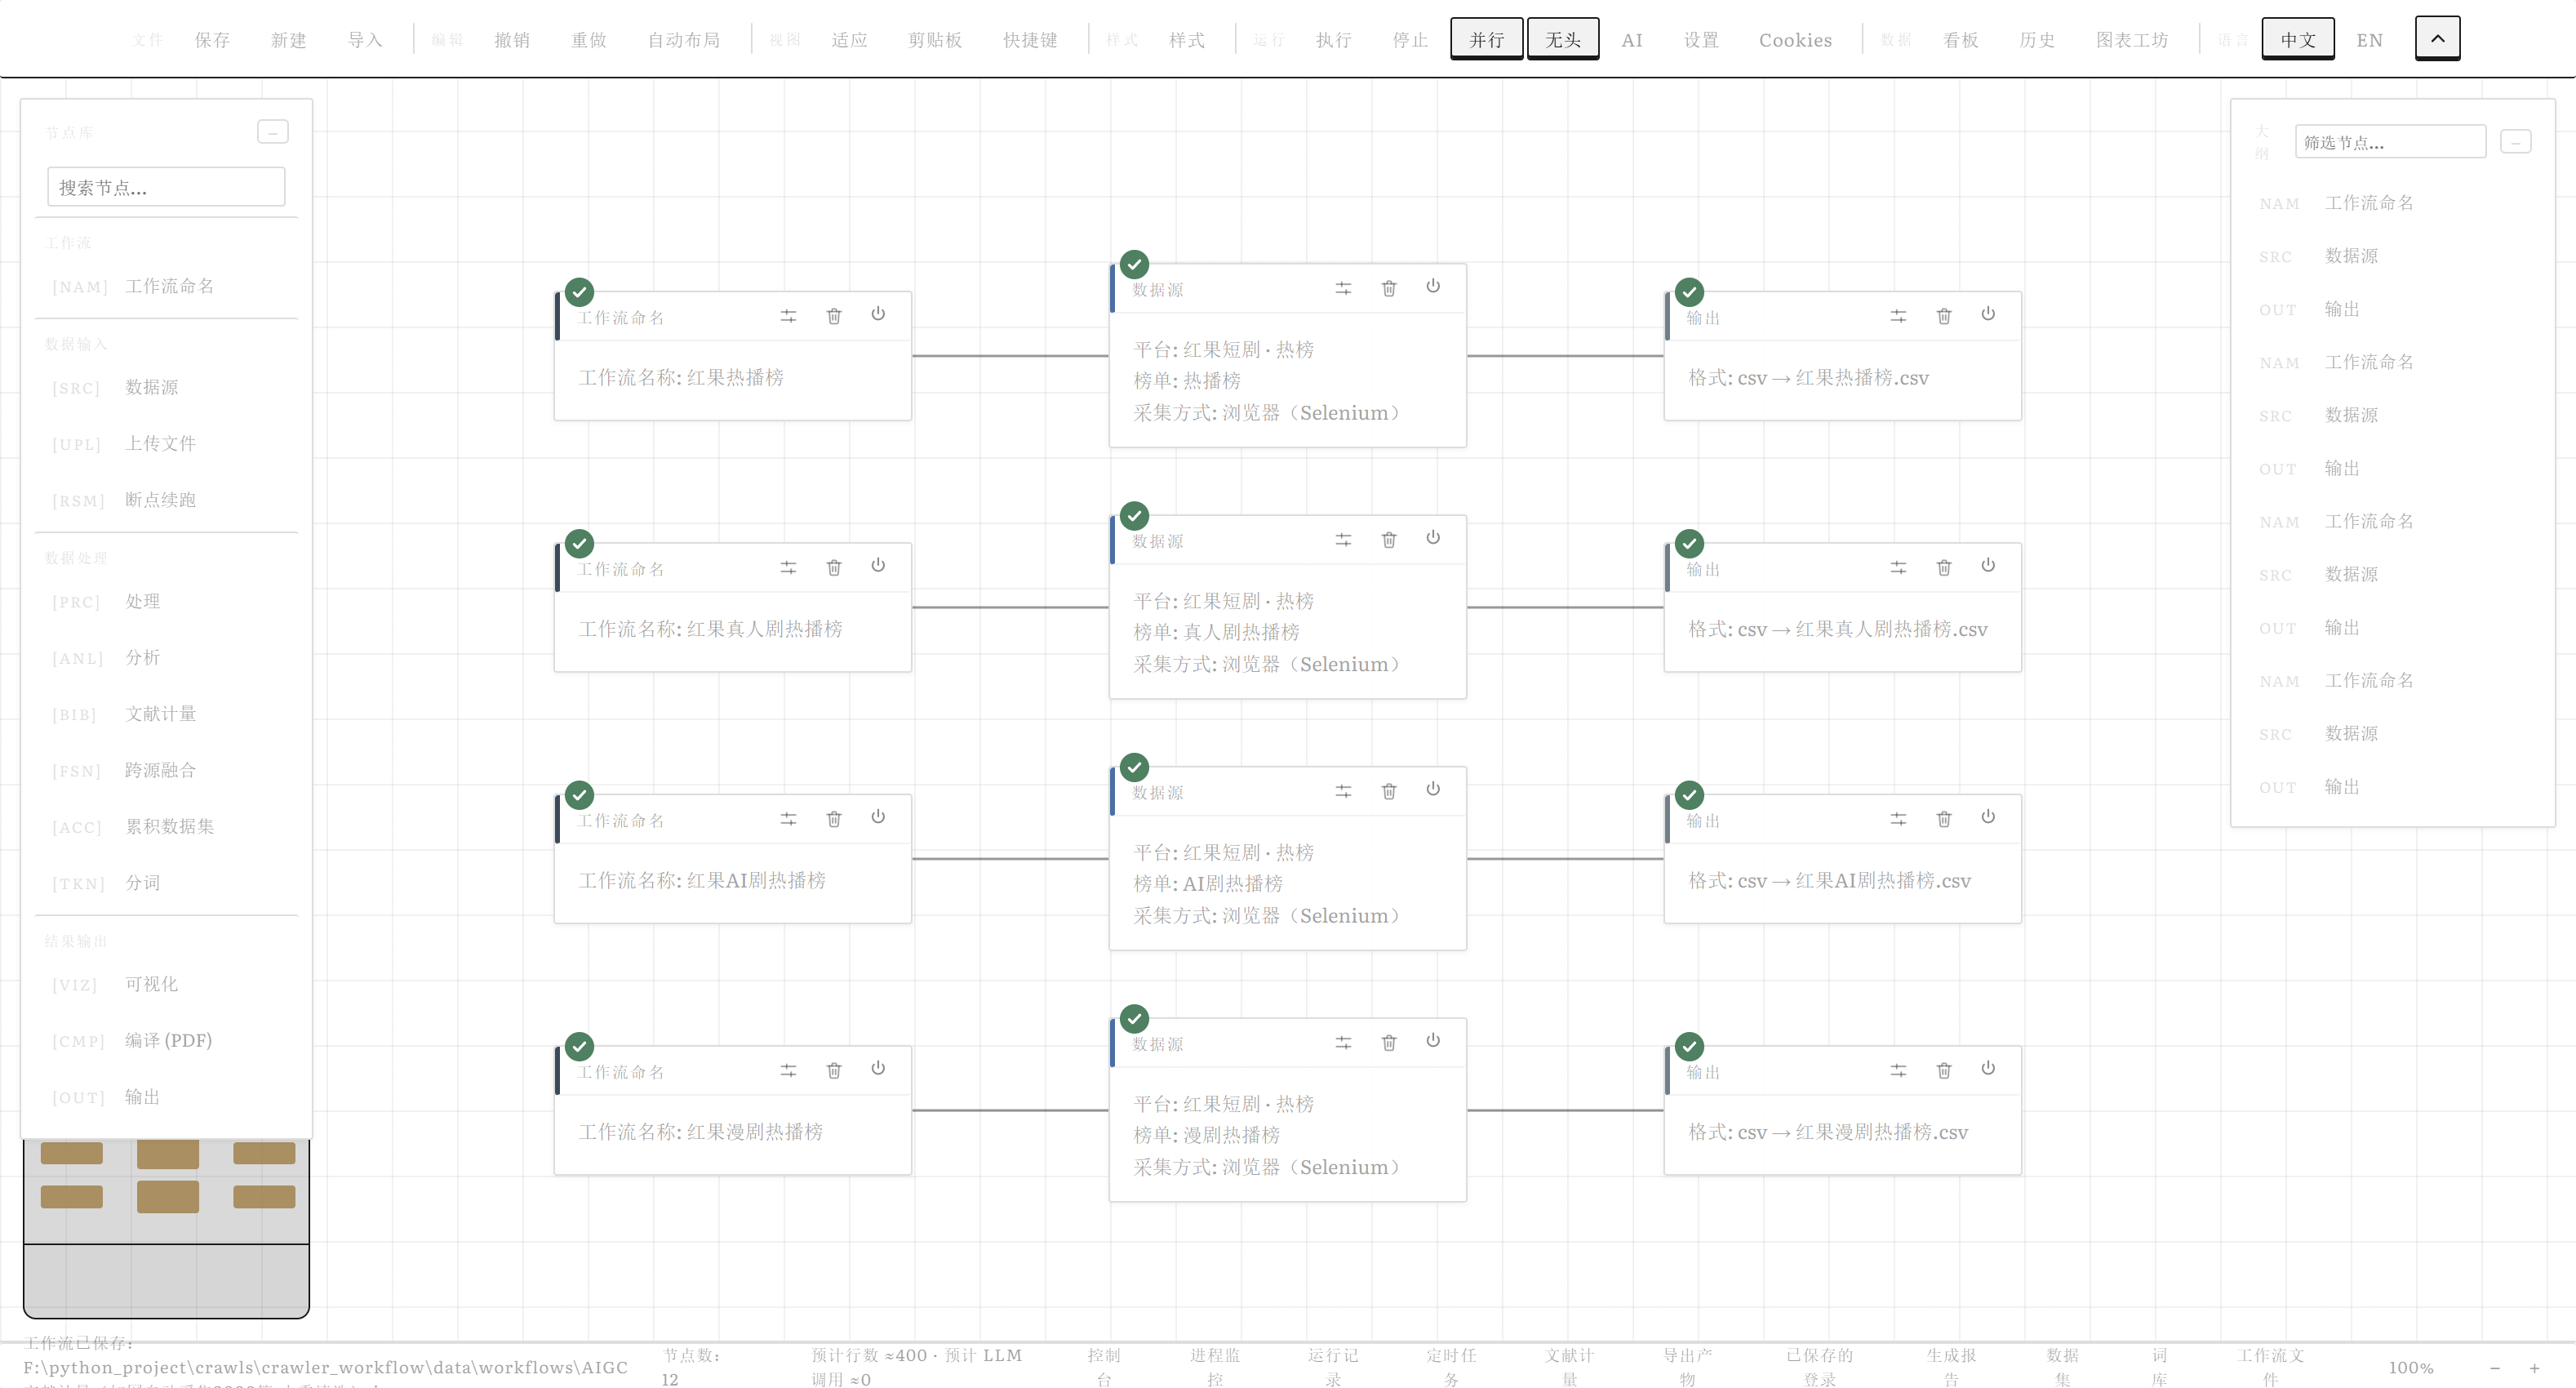
\includegraphics[width=\textwidth]{hg-canvas.png}};
\node[badge,fill=paper] at ([xshift=0.45cm,yshift=-0.40cm]shot.north west) {1};
\node[badge,fill=paper] at ([xshift=0.55cm,yshift=-2.35cm]shot.north west) {2};
\node[badge,fill=paper] at ([xshift=6.9cm,yshift=-2.55cm]shot.north west) {3};
\node[badge,fill=paper] at ([xshift=-1.0cm,yshift=-1.55cm]shot.north east) {4};
\node[badge,fill=paper] at ([xshift=1.05cm,yshift=0.65cm]shot.south west) {5};
\node[badge,fill=paper] at ([xshift=-0.75cm,yshift=0.25cm]shot.south east) {6};
\end{tikzpicture}
\caption{界面的六块区域，画布里是一份跑过的红果工作流}
\label{fig:ui-map}
\end{figure}

\subsection{大纲}

大纲按画布顺序列出每个节点，左边是类型代码，右边是标题。顶部搜索框按标题筛选，点一条就把画布镜头对准它并选中。
面板右上角的减号把大纲折成一条窄边，给画布让出宽度。

\begin{figure}[H]\centering
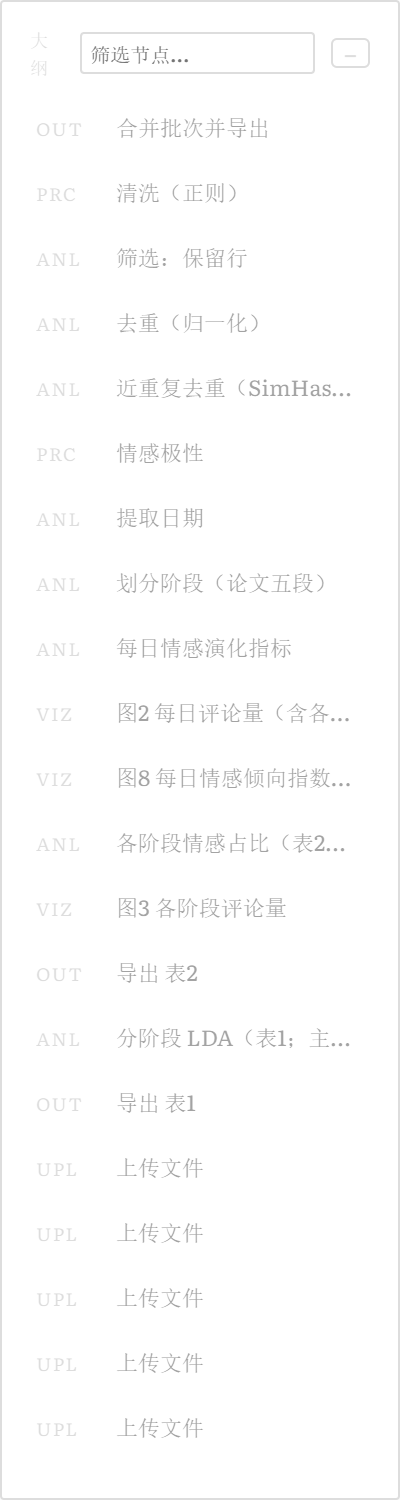
\includegraphics[width=0.43\textwidth]{outline.png}
\caption{大纲：搜索、类型代码、标题，点一条跳过去}
\label{fig:outline}
\end{figure}

\subsection{停靠面板}

底部一行按钮各管一个面板。面板从底部升起，占屏幕下半部分，再点同一个按钮收起。每个面板的内容都是服务端现算的，
所以看到的是这一刻的真实状态，不是页面打开时的旧快照。

\begin{table}[H]\centering
\caption{停靠面板一览}
\label{tab:docks}
\small
\begin{tabularx}{\textwidth}{p{2.6cm}X}
\toprule
面板 & 内容 \\
\midrule
控制台 & 本轮运行的实时日志，按工作流分页签，可按级别过滤、搜索、下载 \\
进程监控 & 服务内正在跑的后台线程，看得出哪个采集卡住了 \\
运行记录 & 每次运行的状态、节点数、行数、耗时，能载入某次结果、看日志、出报告、删除 \\
定时任务 & 按天、按周、按间隔或 cron 定时执行一张已存画布 \\
文献计量 & 已建网项目的快照与跨运行对比 \\
导出产物 & 所有落盘文件，下载、删除、复制路径 \\
已保存的登录 & 每个平台每个账号的 Cookie 与浏览器目录 \\
数据集 & 上传过的表格，来源、列数、行数、被谁引用 \\
词库 & 停用词与领域词 \\
工作流文件 & 打开、重命名、导入导出、打包成项目 \\
\bottomrule
\end{tabularx}
\end{table}

\begin{figure}[H]\centering
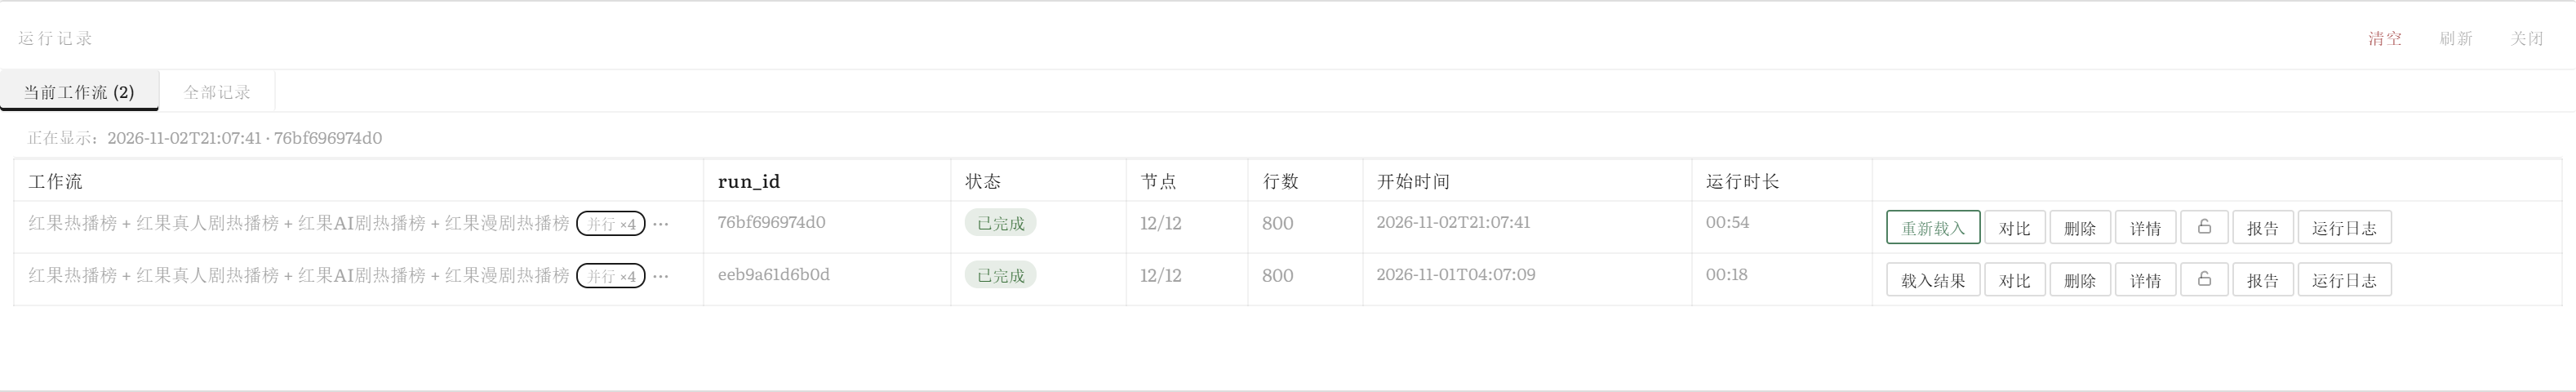
\includegraphics[width=0.98\textwidth]{runs-panel.png}
\caption{运行记录：状态、节点数、行数、耗时与每一行的操作}
\label{fig:runs-panel}
\end{figure}

\begin{figure}[H]\centering

\includegraphics[width=0.43\textwidth]{datasets.png}
\caption{数据集面板，一份表格一行}
\label{fig:datasets}
\end{figure}

\subsection{样式}

菜单条的“\texttt{样式}”管三件事：背景、主题、排布，另加一个圆角滑杆。背景有五档由浅到深的底纹，
主题有自动、浅色、深色三档，自动跟随系统。排布选“\texttt{算法排布}”按连线分层摆放，
选“\texttt{布局基准}”恢复你为这份工作流存过的位置；基准要先保存工作流才能选。
“\texttt{打开画布历史}”给当前状态起名存档，一次最多一百份，恢复之前列出与当前状态的差异，恢复本身也算一步撤销。

\begin{figure}[H]\centering
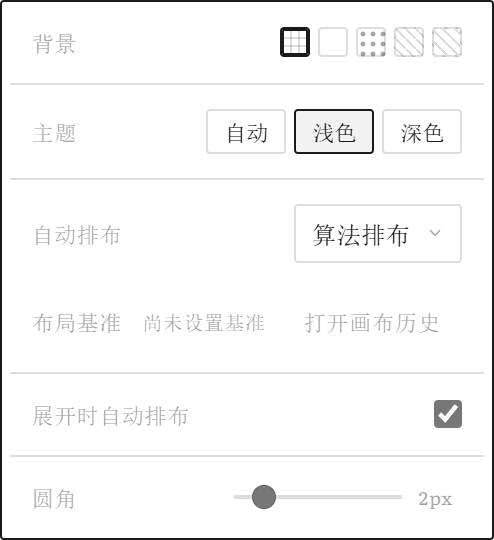
\includegraphics[width=0.5\textwidth]{style-menu.png}
\caption{样式菜单：背景、主题、排布、布局基准、画布历史、圆角}
\label{fig:style-menu}
\end{figure}

\section{画布}

画布是一张可以无限大的桌面。下面十个动作覆盖日常九成操作。

\begin{enumerate}
\item 放节点。点节点库的条目，或者按住拖到画布上松手。新节点落在视野中央或落点。
\item 连线。鼠标移到节点右侧的小圆点，按住拖到下一个节点左侧的圆点，松手成线。
\item 删除连线。点一下线，线变粗，按 Delete；框选可以一次删多条。
\item 选中。单击选一个，Shift 加单击加选，空白处拖方框框选。
\item 移动。拖节点本身；方向键逐像素微调，按着 Shift 步子更大。
\item 缩放与平移。滚轮缩放，空白处拖动平移，“\texttt{适应}”把所有节点装回屏幕，缩略图点哪去哪。
\item 撤销重做。菜单条的两个箭头，也可以按 Ctrl 加 Z。参数、挪位、连线都算一步。
\item 禁用节点。节点右上角的电源按钮。关掉以后不参与运行，下游失去唯一输入的节点也一起失效。
\item 复制粘贴。Ctrl 加 C 与 Ctrl 加 V，副本参数一样，位置稍微错开；剪贴板面板跨页面保存复制过的节点与文本。
\item 命名与注释。“\texttt{工作流命名}”给这一段起名字，运行记录和日志就用这个名字；“\texttt{注释}”节点不参与数据，只在画布上写说明。
\end{enumerate}

\begin{figure}[H]\centering
\begin{tikzpicture}[scale=0.95]
  \node[card=src,minimum width=3.0cm] (n1) at (0,0) {数据源};
  \node[card=prc,minimum width=3.0cm] (n2) at (4.6,0) {清洗};
  \draw[wire] (1.55,0) -- (3.05,0);
  \fill[src] (1.55,0) circle (2.4pt);
  \fill[prc] (3.05,0) circle (2.4pt);
  \draw[draw=ink!18,line width=0.4pt] (1.55,0) circle (5.5pt);
  \draw[draw=ink!18,line width=0.4pt] (3.05,0) circle (5.5pt);
  \node[micro,above=8pt] at (2.3,0.5) {拖住右侧圆点，落到左侧圆点};
\end{tikzpicture}
\caption{连线的两个圆点}
\label{fig:wire}
\end{figure}

快捷键都写在“\texttt{视图}”里的“\texttt{快捷键}”面板上：Enter 开合节点面板，L 进入连线模式，WASD 在节点之间跳，
空格加拖动平移，Delete 删除选中，Ctrl 加 Z 撤销，Ctrl 加 F 跳到大纲搜索。面板里列出的组合就是画布真正绑定的那一组。

\begin{figure}[H]\centering
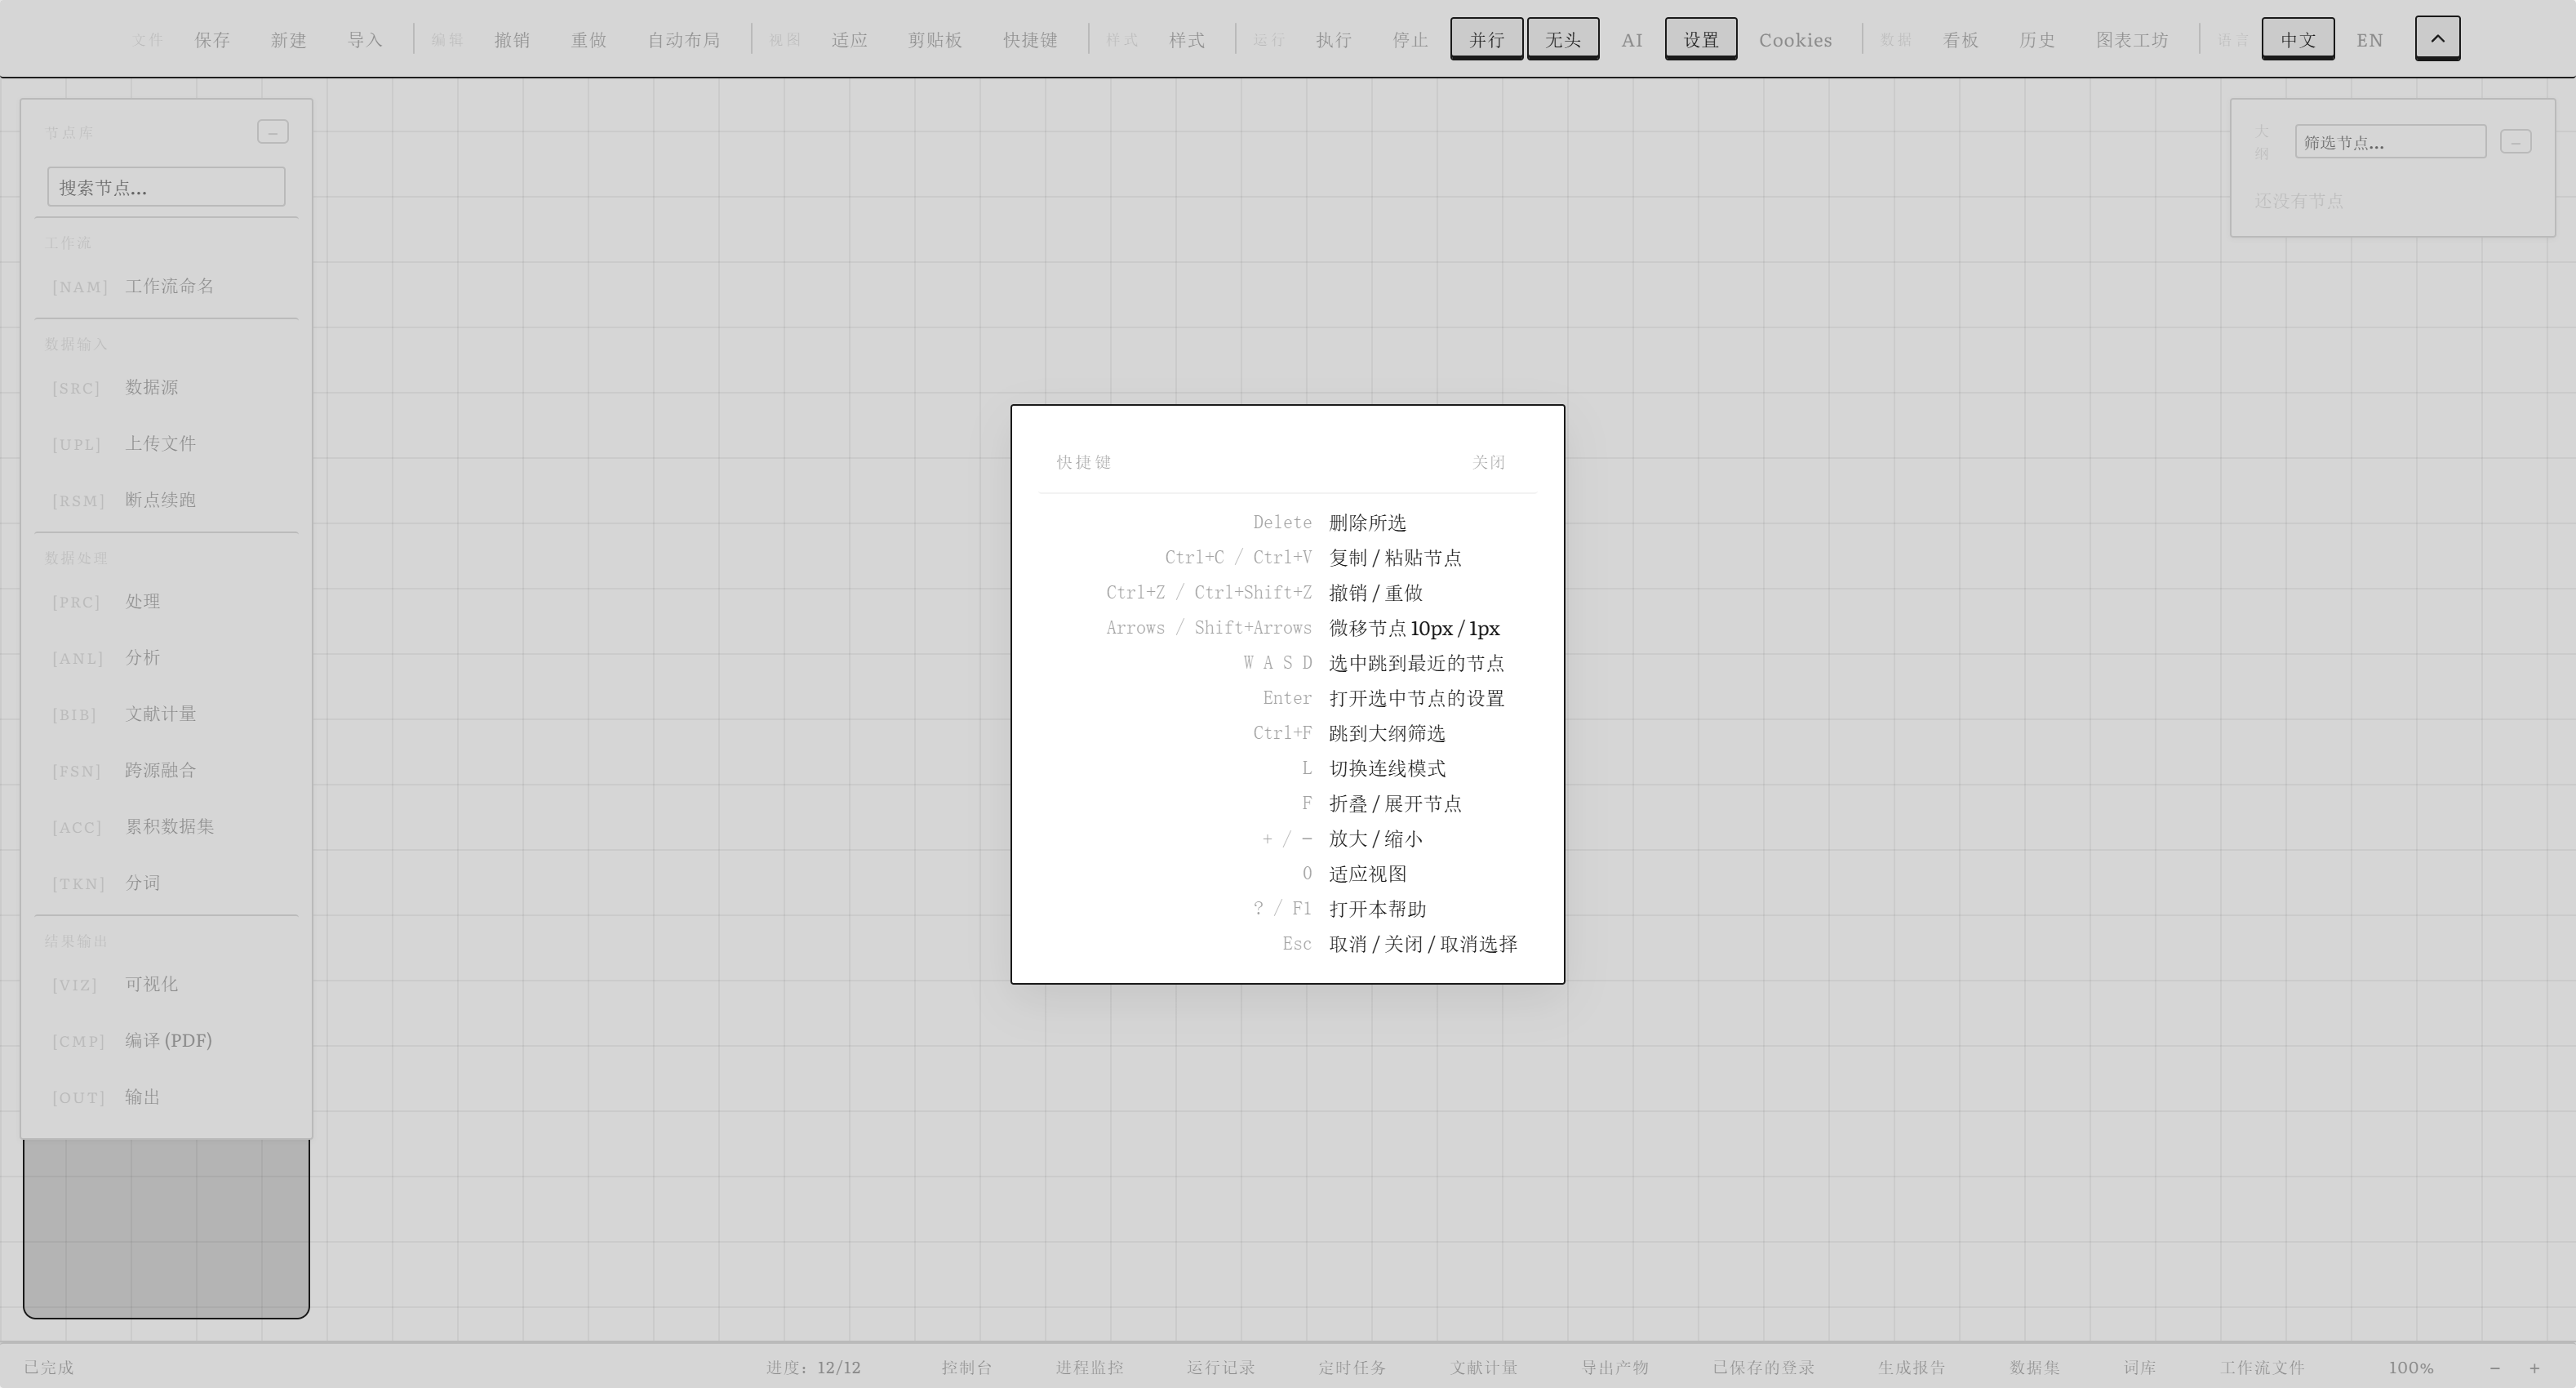
\includegraphics[width=0.72\textwidth]{shortcuts.png}
\caption{快捷键面板}
\label{fig:shortcuts}
\end{figure}

复制过的节点与文本进“\texttt{剪贴板}”抽屉，按标题或内容搜索，可以置顶、改名、单条删除或清空。抽屉里的内容重启浏览器还在。

\begin{figure}[H]\centering

\includegraphics[width=0.5\textwidth]{clipboard.png}
\caption{剪贴板抽屉}
\label{fig:clipboard}
\end{figure}

\section{节点与参数面板}

节点长得都一样：左边一道竖色条表示类型，标题下一行摘要写关键参数，右边三个按钮，依次是设置、删除、开关。

\begin{figure}[H]\centering
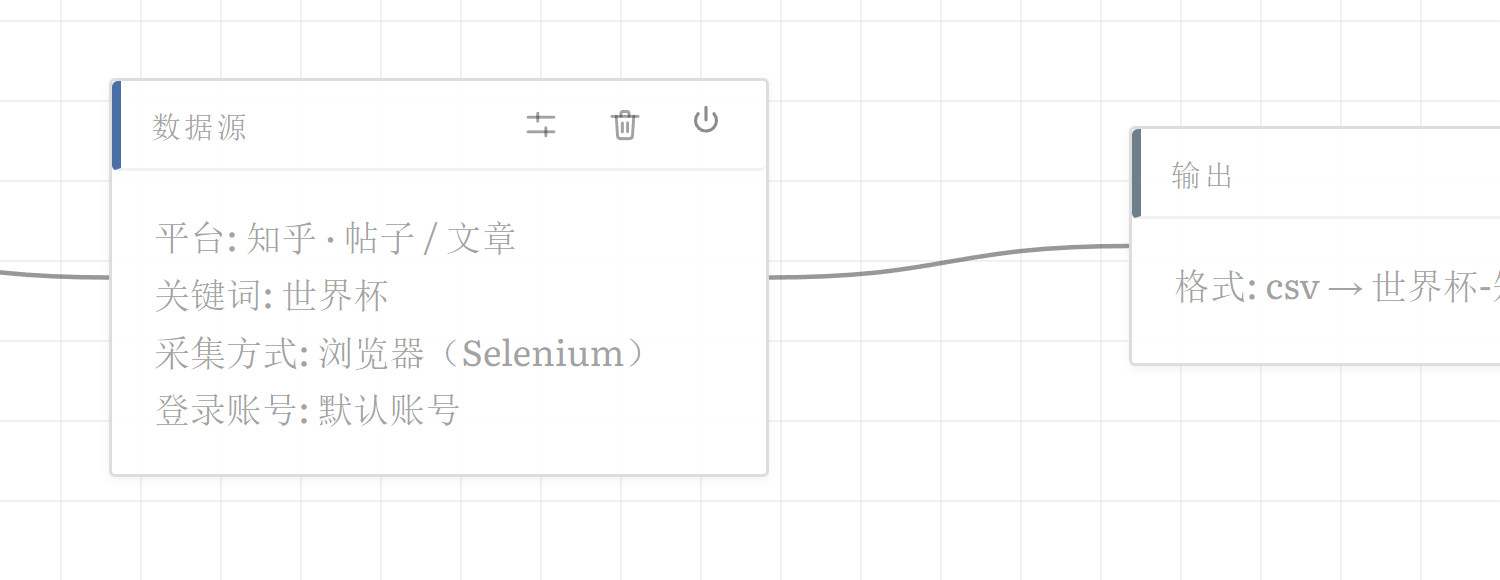
\includegraphics[width=0.72\textwidth]{node-closeup.png}
\caption{一个数据源节点：设置、删除、开关}
\label{fig:node}
\end{figure}

右上角还有状态角标。绿勾是完成或复用了以前的结果，转圈是在跑，红叉是没成功，灰色小点是没跑过或被关掉。
角标只反映运行库里的结论，不会把没跑过的画成成功。

点设置按钮打开右侧参数面板。面板结构固定：顶上写节点类型与标题，接着是这一段运行的校验结论，下面是主参数，最下面是预览按钮。
每一行都对应一个数据列或者一个行为；凡是需要先选一项才能继续的字段，面板不替你猜默认值，选错会按名字拒绝并列出可选项。

\begin{figure}[H]\centering
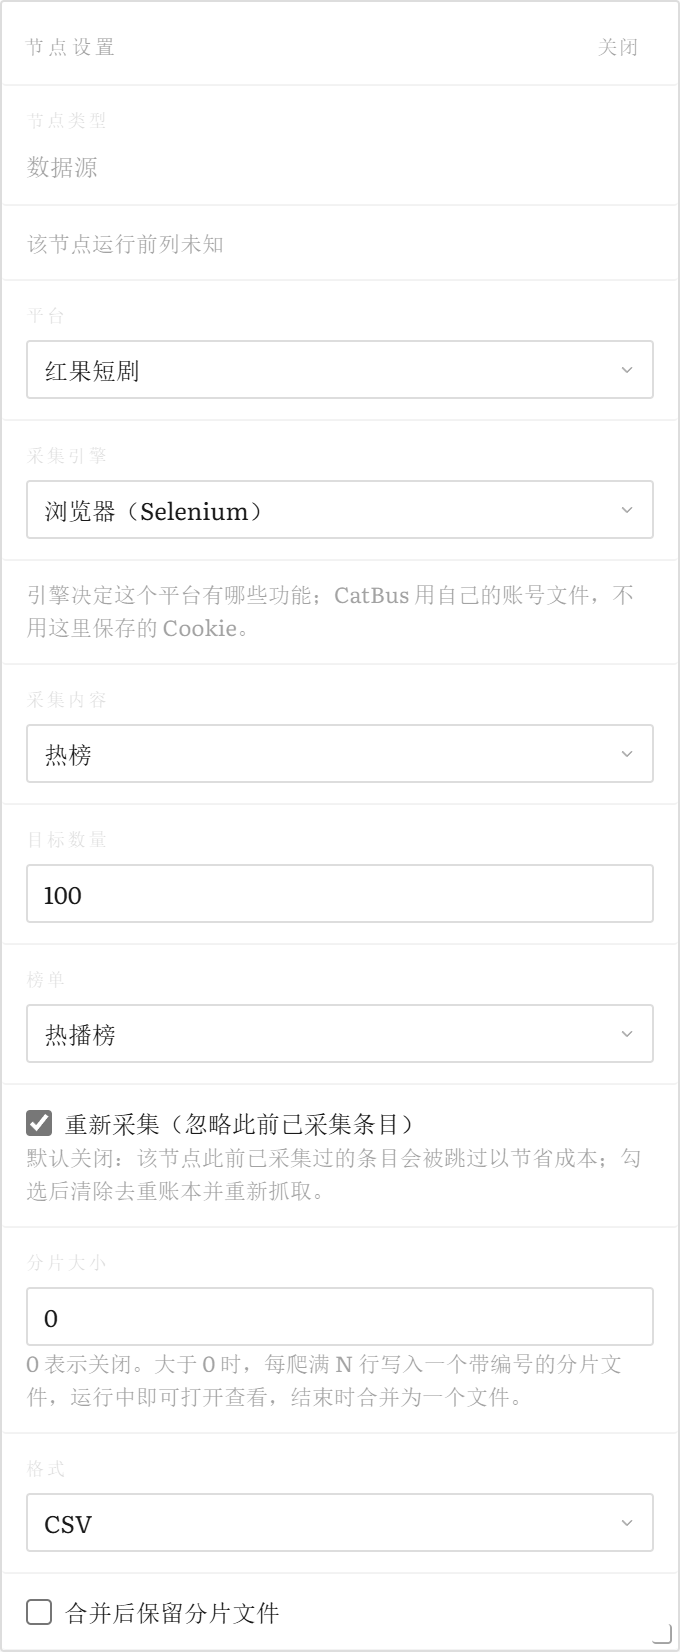
\includegraphics[width=0.31\textwidth]{panel-source.png}
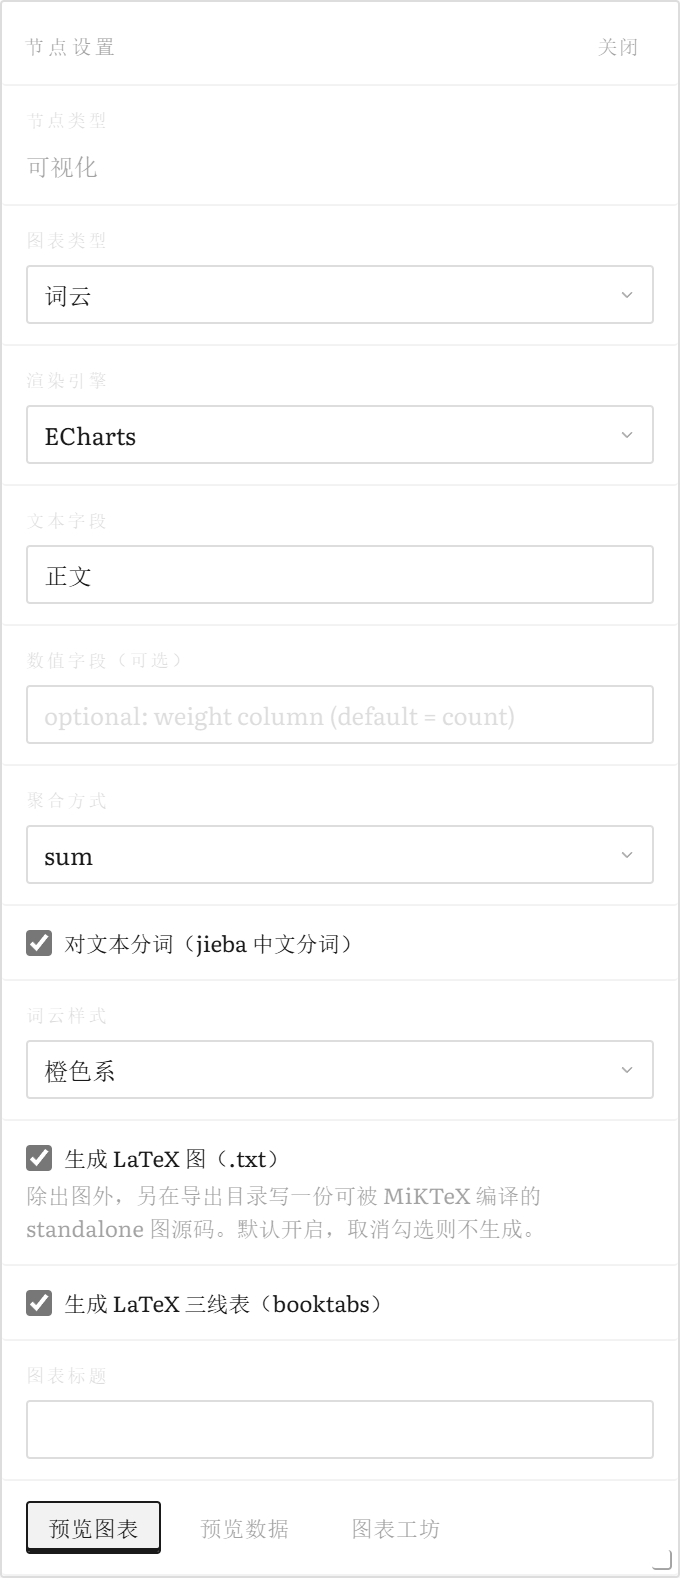
\includegraphics[width=0.31\textwidth]{panel-visualize.png}
\caption{左：数据源面板，平台、内容、数量、格式往下排；右：可视化面板，图表类型、引擎、字段、标题}
\label{fig:panels}
\end{figure}

摘要行值得常看。数据源写平台、内容、关键词或链接、账号；上传写文件名与行数；分析写操作与输出列；
可视化写图表类型与标题；输出写格式与文件名。看一眼摘要就知道这个节点是不是上次调好的那一份。

\section{节点类型}

节点库十三种，按数据流分工。

\begin{table}[H]\centering
\caption{节点类型}
\label{tab:nodes}
\small
\begin{tabularx}{\textwidth}{p{2.4cm}X}
\toprule
节点 & 作用 \\
\midrule
工作流命名 & 给这一条链贴名字，运行记录与日志用它 \\
数据源 & 采集一个平台的一种内容 \\
上传文件 & 读一张本地表，或挂一份已存数据集 \\
断点续跑 & 把历史运行的输出行收回来当输入，不重新采 \\
处理 & 分词、清洗、情感、倾向、关键词、聚类、实体、网暴、水军、相关、显著、异常 \\
分析 & 去重、筛选、选列、改名、排序、采样、聚合、关联、分箱、时间、阶段、主题、演化、预警 \\
文献计量 & 题录建网、指标、聚类、突现、变异、叠加 \\
跨源融合 & 多张表折成一份规范表 \\
累积数据集 & 每次追加新行到带版本的长期表 \\
可视化 & 三十种图与十四类文献图谱，另出 LaTeX 图源 \\
编译 & 把图和表用本机 xelatex 编成 PDF \\
输出 & 落成 CSV、JSON、Excel、文本、HTML、Markdown、Parquet 或 PDF \\
\bottomrule
\end{tabularx}
\end{table}

\begin{figure}[H]\centering

\includegraphics[width=0.31\textwidth]{panel-upload.png}
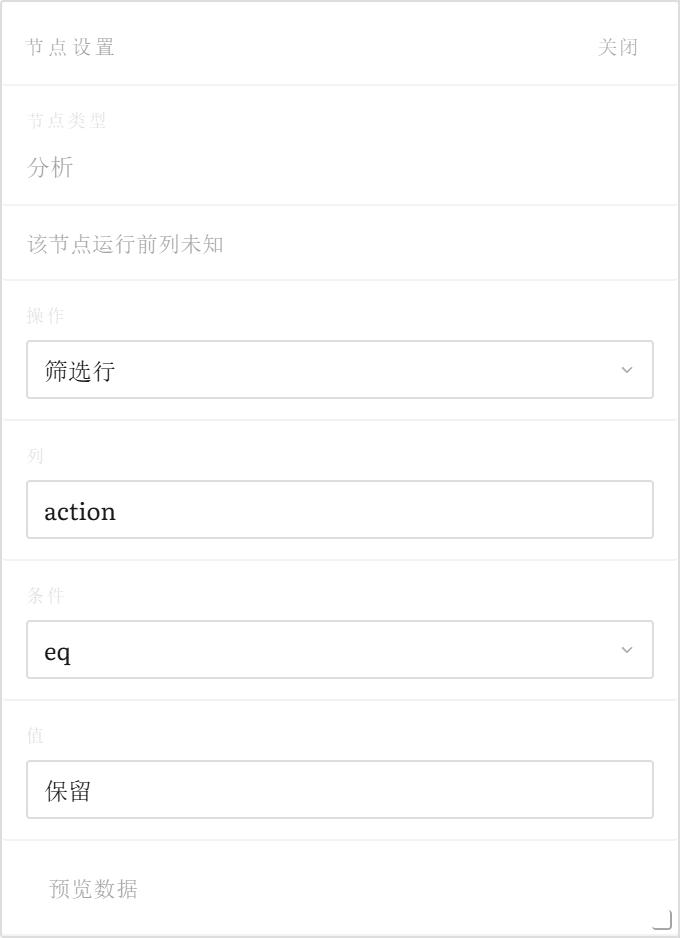
\includegraphics[width=0.31\textwidth]{panel-analysis.png}

\includegraphics[width=0.31\textwidth]{panel-output.png}
\caption{上传、分析、输出三个面板，字段都按上游实际列名给候选项}
\label{fig:panels2}
\end{figure}

\section{运行一次}

按下“\texttt{执行}”先做三项检查：画布有没有环，每个节点参数齐不齐，这次要用的平台有没有登录状态。
任何一项不过就在开始前停下，控制台写清是哪个节点哪一项。

检查通过以后按连线顺序跑。一个节点可以接多个上游，上游表按列名取并集合并；也可以分给多个下游，各拿一份同样的输入。

服务同一时刻只跑一轮。忙的时候按钮变成“\texttt{排队运行}”，任务进队列，当前这轮结束自动开始。
勾了“\texttt{并行}”，几条互不相连的链同时跑；同一条链里的节点仍然一个接一个。
“\texttt{无头}”让浏览器在后台跑，不占桌面，第一次调试可以不开。

停止按钮把正在跑的与还没跑的节点一起停下。已经写进库的行保留，节点标成停止，不算失败，下次可以从那里接着做。

控制台按工作流分页签，实时输出，刷新页面会重新接上。日志同时写进运行库，事后在运行记录里还能翻到同一份。
进程监控列出服务内正在跑的后台线程，采集卡住时用它看是哪一条。

\begin{figure}[H]\centering
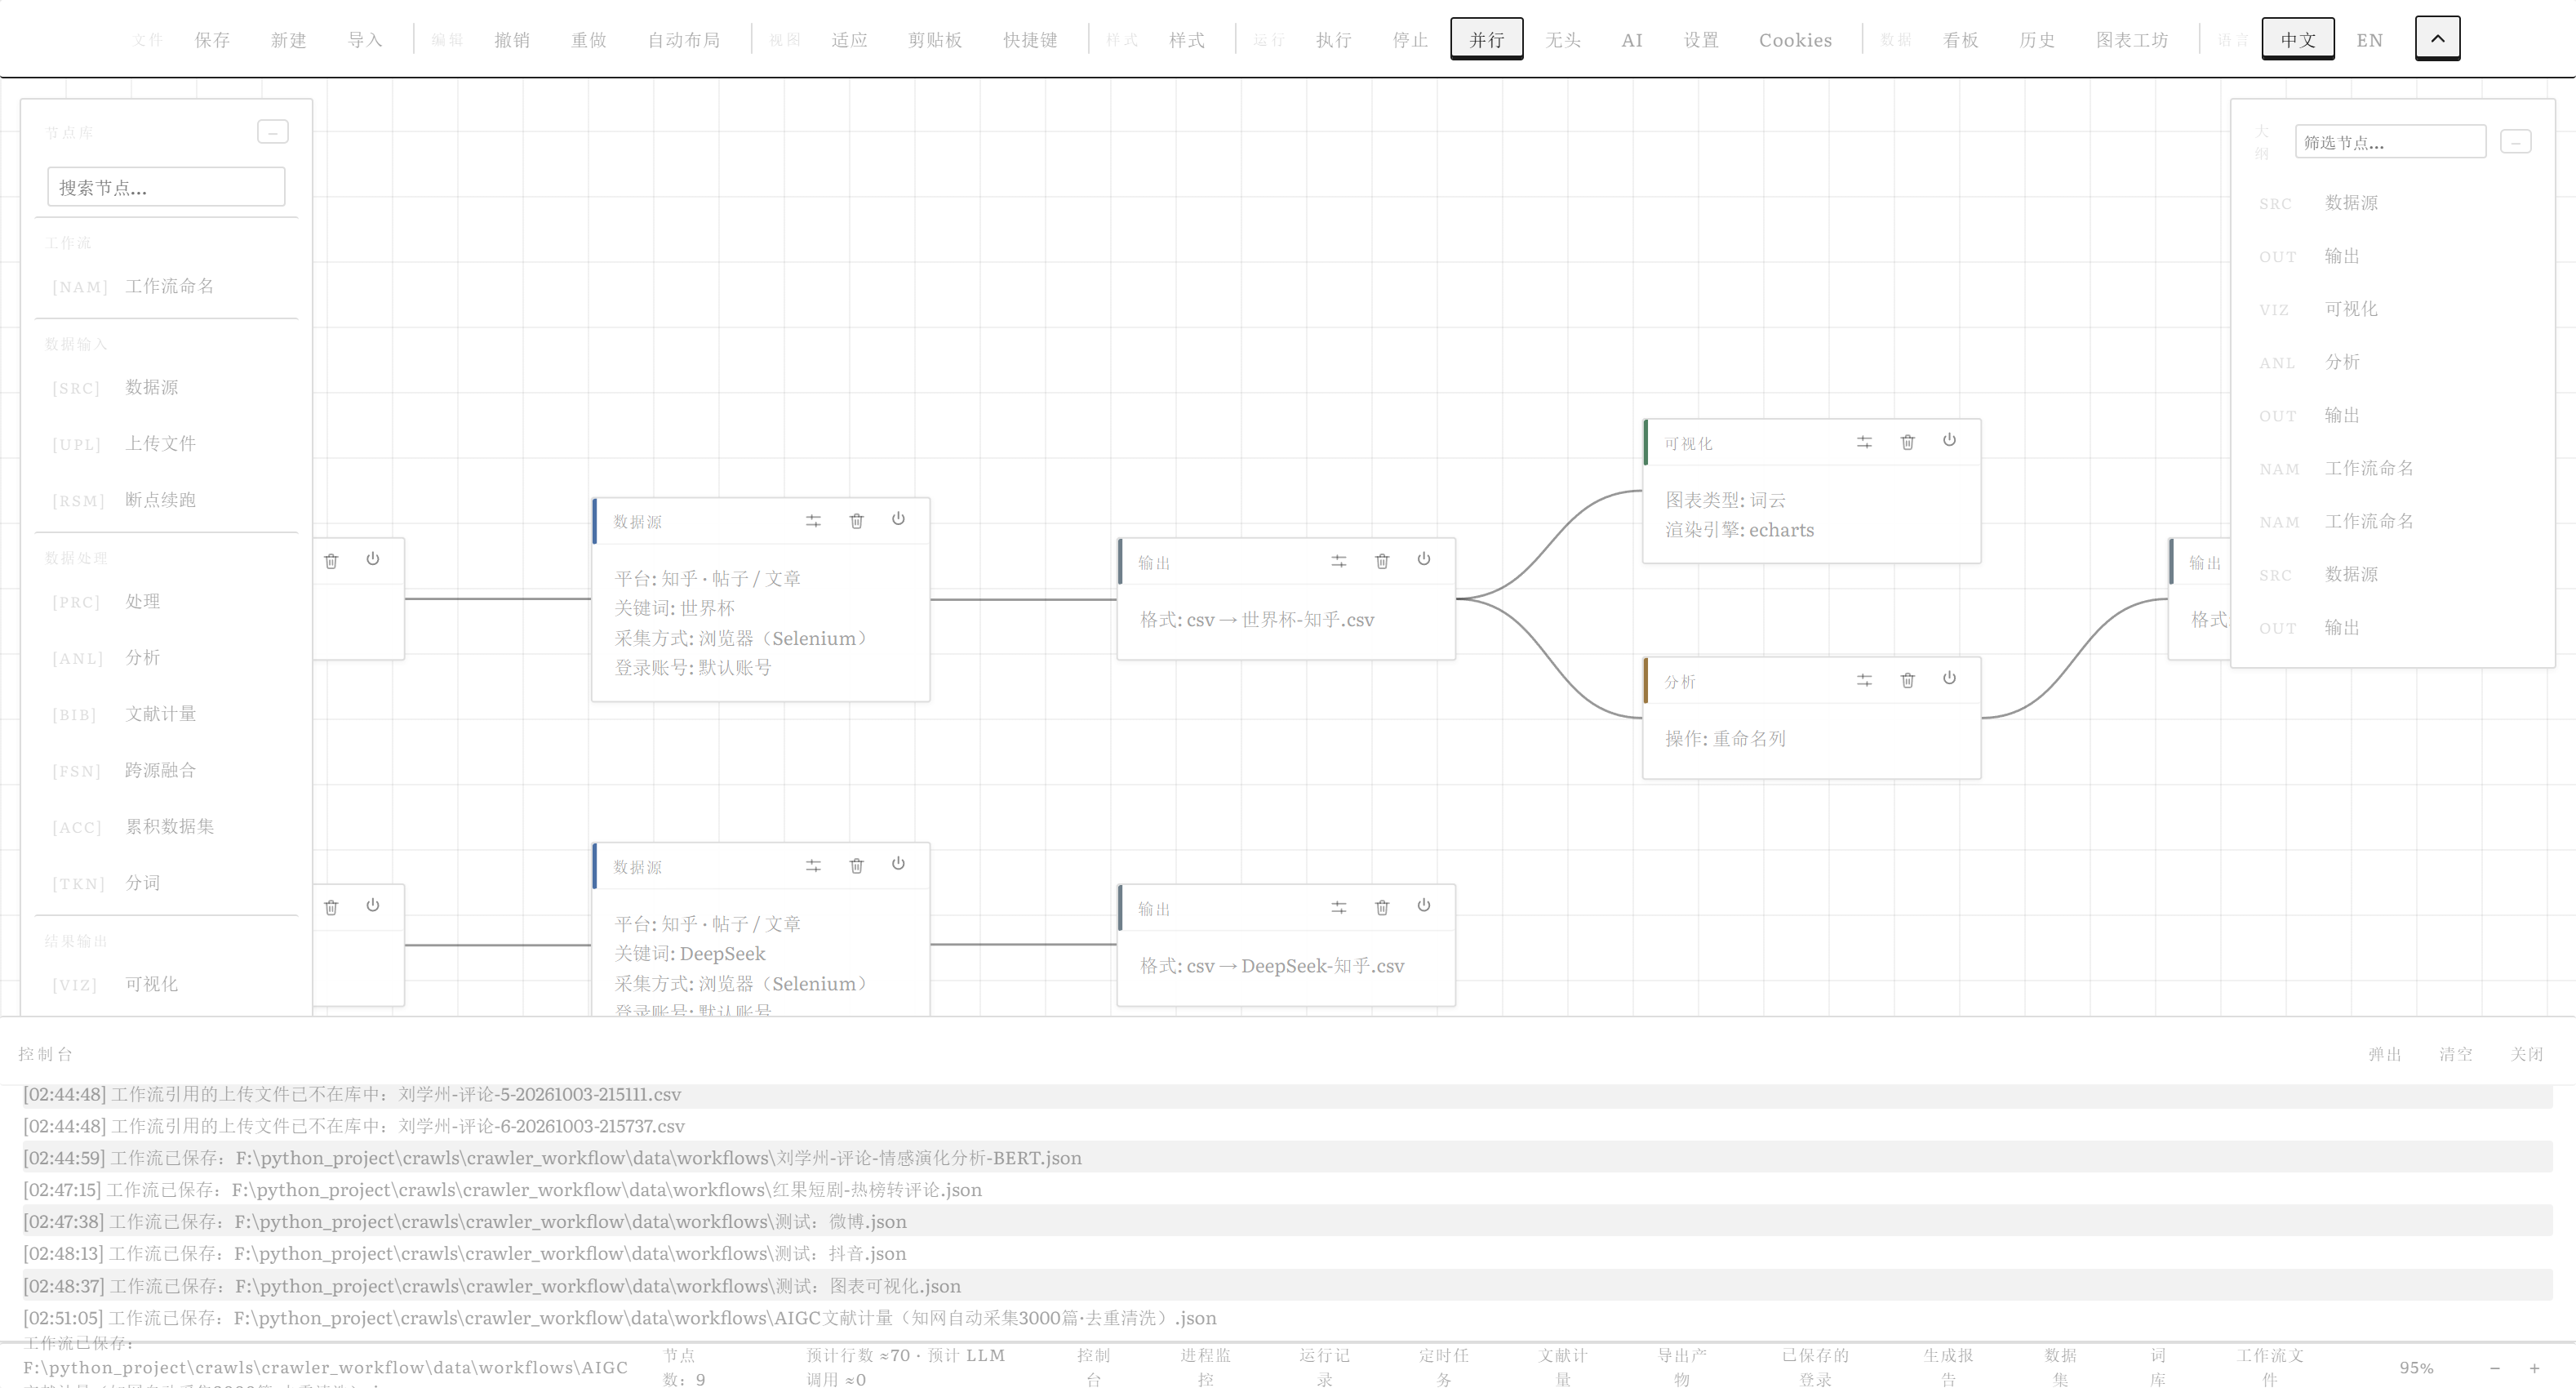
\includegraphics[width=0.98\textwidth]{console.png}
\caption{控制台：工作流页签、级别过滤、搜索、导出}
\label{fig:console}
\end{figure}
